\section{Functional importance of \tgfbsf\ and Wnt signal integration}
\label{pathways:wntTgfb:function}


Having covered the canonical \tgfbsf\ and Wnt signaling pathways, we
can now move forward to the topic of this dissertation: inter-pathway crosstalk.
The goal of this section is to both motivate the study of Wnt/\tgfbsf\
crosstalk and to review the work that has been done in this field.
There are many systems in which both of these pathways are intensively
studied (indeed entire
textbooks have been written on these pathways). However, most of this work
studies each pathway indepenently; there exists a much
smaller body of work on Wnt/\tgfbsf\ inter-pathway
crosstalk. One of the more experimentally-tractable of such systems is the
adult mammalian gut, and so I focus my review on this system.


The study of adult stem cells has advanced rapidly in recent years,
especially with the identification of resident stem cells for several
tissues \cite{Barker2010} and with the discovery that differentiated
cells can be turned pluripotent by expression of a handful of
transcription factors \cite{Takahashi2006}.
However, there is still much that we do not understand about stem
cell biology in general, especially because \i{in vitro} studies
are difficult to map back to \i{in vivo} phenomena,
and because each stem cell system has proven to have its own quirks including
differential use the same genetic pathways.


In particular, work in this field has
pointed toward \tgfbsf\ signaling being a major factor in stem cell
differentiation, while canonical Wnt signaling seems to control stem cell
maintenance. There are cases where this oppositional role assignment does not occur
\cite{VonBubnoff2001,Fischer2002,Nakashima2005,Itasaki2010a,
Feigenson2011,Lander2012,Malhotra2009,Davidson2012}, though
it is fairly common across stem cell systems
\cite{Verheyen2010,Libusova2010,Gregorieff2005,VandeWetering2002,
Schepers2012,Teo2006}. These roles are
particularly well-studied in the context of the mammalian intestine.


Our understanding
of the intestinal stem cell system has increased significantly in recent years,
due in no small part to the work of Hans Clevers and colleagues.
Clevers' group has dissected the function of many genes involved with
intestinal stem cell development (with a focus on canonical Wnt), has
unambiguously identified the stem-cell population \cite{Barker2007a},
and has developed an \textit{in vitro} system for culturing intestinal
stem cells in such a way that they behave like homoestatic \textit{in vivo} crypts
\cite{Sato2011a,Sato2011b}. This work has even led to successful engraftment
of intestinal stem cells isolated from one mouse into the damaged
intestine of another \cite{Yui2012}. Given the potential value to stem
cell therapy, and the connection of stem cells with colon cancer
\cite{Zeki2007,Barker2009a}, a deeper understanding of intestinal stem
cells is highly sought after in hopes of obtaining new therapeutic strategies
for many bowel diseases.


While the gut stem cell system is highly studied, it is poorly understood
how intestinal stem cells
integrate distinct signals from their environment, such as Wnt and \tgfbsf,
and thus choose one of several differentiated outcomes. Given the oppositional
roles of \tgfbsf\ and Wnt in the gut, and their various functional interactions in other systems
\cite{Attisano2004,Labbe2007,Chong2009,Itasaki2010a,Minoo2010a,
Serra2011,Feigenson2011,Rodriguez-Carballo2011,Chen2012a,Akhmetshina2012,Song2014},
it is important to understand generally how cells integrate these two signals.


\subsection{\tgfbsf\ and Wnt in the intestinal crypt}
\label{pathways:wntTgfb:gut}

\subsubsection{Crypts are the functional unit of intestinal epithelium}

The small and large intestine both contain
similar stem cell systems. Between these two organs, morphological
differences in stem cell systems are revealing in terms of the distinct organ functions.
The small intestine contains a high fraction of absorptive cells (enterocytes)
and an increased epithelial surface area due to relatively large lumenal projections termed
villi, consistent with its role in digestion and absorption of food.
The colon is predominantly made up of mucus-secreting goblet cells
and completely lacks villi, consistent with its need to carry potentially
abrasive and toxic waste \cite{Iacopetta2002}. The protective role of
goblet cells is highlighted by the connection between goblet cell
loss and rapid tumor formation in mice \cite{Yang2008}. The colon is of
particular clinical interest due to the high rates of cancer
and inflammatory diseases of this organ \cite{Jemal2010}. Despite macroscopic differences
in morphology, many aspects of of the stem cell biology seem to be similar
in the small and large intestine.


A cross-section of the intestine would reveal a hollow tube whose wall
consists of several tissue layers. The
most-lumenal layer consists of the mucosa, a single sheet of epithelium
over stromal tissue (fibroblasts, collagen, blood/lymphatic vessels, etc.),
together forming crypts and their support structures.
The epithelium sits atop a basement membrane
\cite{Simon-Assmann2010} which in turn is immediately adjacent to
myofibroblasts such that each crypt is essentially sheathed in these cells.
Though it is likely that important signaling takes place between the
epithelium and stroma \cite{Simon-Assmann2010,Kosinski2010,Ingham2011},
these signals are difficult to study and their importance is unclear given
the fact that \i{ex vivo} isolated crypts maintain a differentiating,
homeostatic structure even in the
absence of a macroscopically polarized stroma \cite{Sato2011a,Lahar2011}.


The crypts are the functional unit of the intestine. The single epithelial layer
of each crypt contains only
$\sim$10 stem cells at the base that divide on average once per day,
generating a conveyor belt of rapidly dividing and differentiating cells
\cite{Snippert2010} \arp{fig:pathways:crypt}. These ``transit amplifying'' cells stop dividing
after full differentiation and are eventually lost to the lumen of the gut
\cite{Eisenhoffer2012}. This process is fast, such that the entire non-stem
cell population of a crypt is turned over every 3-5 days \cite{Buske2011}.


In the small intestine, the top of the crypt (which is the base of
the villus) is roughly the point at which cells are completely differentiated.
Note that this generally accepted model of crypt turnover
is based on studies of the small intestine and is thought to be similar in
the colon, though there are important
differences between the organs that should be considered.
For example, the large intestine completely lacks the paneth cells that have
recently been reported to be required for stem cell maintenance in the small
bowel. However, colonic crypts do contain cells
expressing similar surface proteins \cite{Sato2011b}.
Additionally, the entirety of the colonic crypt contains apparently-differentiated
cells, suggesting that the transit amplifying population
is much smaller than in the small bowel.
On the other hand, the literature generally supports that the population
dynamics and signaling factors are similar between the small and large
intestine, and between mouse and human.


	\begin{figure}%[ht]
	\centering
	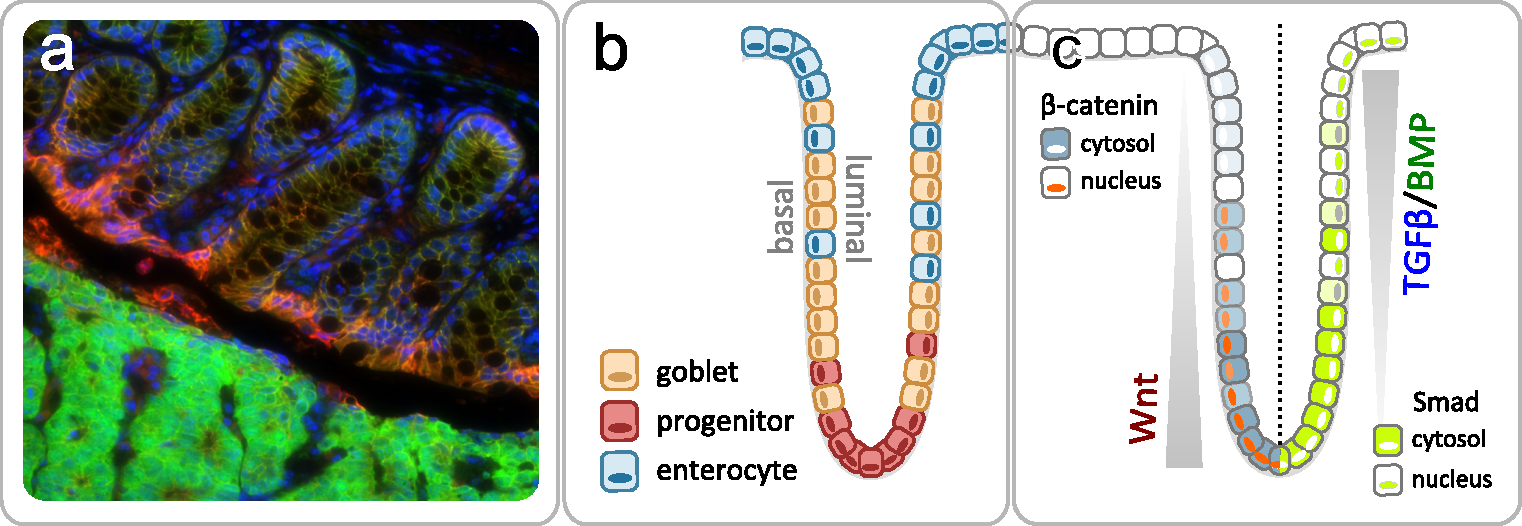
\includegraphics[width=6in]{FIGS/pathways/crypt.pdf}
	{\singlespacing 
	\caption[Expression patterns of Wnt and \tgfbsf\ in colonic crypts]
            { Overview of \tgfbsf\ and Wnt signaling patterns
            in the colonic crypt. \b{a}, Immunostained crypts
            from a CPC;APC mouse \cite{Hinoi2007} showing two opposing sides pinched
            together, with the dark lumen in between. Blue, DNA; green,
            \bcat, red, E-cadherin. The bottom set of crypts are tumorous;
            note the global increase in \bcat. Image curtesy Michael
            Ramirez and Curtis Thorne (Altschuler \& Wu lab,
            Univeristy of Texas Southwestern).
            \b{b}, Cartoon of colonic crypt
            structure, showing key cell types. \b{c}, Cartoon of
            signaling gradients in the crypt, showing high Wnt
            at the crypt base and high \tgfbsf\ at the crypt tops.}
	\label{fig:pathways:crypt}}
	\end{figure}



\subsubsection{Opposing gradients of \tgfbsf\ and Wnt in crypts}


Within the crypt epithelium, there are distinct patterns of expression for
the Wnts and the \tgfbsf\ ligands that together seem to control cell
fate in a crypt-axis positional manner. Using fluorescence in situ hybridization
(FISH), Clevers' group showed that canonical Wnts and various FZDs were
preferentially expressed in the crypt base, while non-canonical Wnts were
expressed throughout the crypt or only at the top \cite{Gregorieff2005}.
The same group later found that LGR5, a Wnt co-receptor,
is a highly specific marker for intestinal stem cells \cite{Barker2007a}.
This discovery allowed for labeling and purification of this cellular population,
and the demonstration that this cell type alone could
re-create crypt-like structure \i{in vitro}.


There is evidence that the paneth cell population is the source
of canonical Wnt3A in the crypt base \cite{Sato2011b},
though this is confounded by a study showing that this cell
type can be ablated \textit{in vivo} without loss of stem cell maintentance
\cite{Rizk2012}.
In contrast to canonical Wnt, but similarly to non-canonical Wnt,
\tgfbsf\ ligands and receptors are expressed exclusively in the
the differentiated epithelium at the tops of the crypts
\cite{Hardwick2004,Massague1990}
and villi \cite{Yamada2013}. Smad activity is restricted to
the same parts of the crypt \cite{Hardwick2008,Libusova2010}.


How the gradients are established and maintained, especially in the face
of a constanty turning over cell population, is not well understood.
The relatively long lifespans of the paneth cell population
\cite{DeSantaBarbara2003} hint that this
cell type may serve as a sort of anchor for these gradients. Another
potential source of gradient maintenance are the transmembrane ephrin
receptors and their ligands, which seem to be required for proper cell sorting: their
loss results in disorganized cellular positions within colonic crypts.
Intriguingly, these ephrins and receptors are regulated by canonical Wnt signaling,
though how these two phenomena interact is unclear \cite{Batlle2002}.


Importantly, it is unclear whether these gradients actually function as such.
While the gradients could be formed by secreted molecules diffusing over
multiple cell lengths, the relative insolubility of Wnts argues against this.
Indeed, in the developing fly wing and in the vertebrate notochord, there is
recent evidence that diffusion of Wnt is not the mechanism by which it creates
gradients \cite{Alexandre2014,Serralbo2014}. Additionally, because Wnt and \tgfbsf\
have so many extracellular antagonists, the presence of a ligand gradient is neither
required nor sufficient to have a functional gradient \cite{Wakefield2013}.


\subsection{Wnt drives stem cell maintenance; \tgfbsf\ drives differentiation}

While the opposing gradients of these two pathways hint at
opposing functional roles, they do not imply it. 
The gradients could be a macroscopic consequence of cell sorting.
Or, the gradients could be a marker of crypt position without exerting any
concentration-dependent influence.
The biological argument that most favors truly oppositional roles is that
modulation of one pathway, experimentally or in the context of disease,
is generally paired with opposite deviations of the other pathway.
I reviews examples of this below.


\subsubsection{Increased Wnt signaling is a driver of colon cancer}

It is well established, and has been for some time, that over-activation of
canonical Wnt is a primary force in colon cancer. Multiple components of
the pathway have been implicated in this disease, though clearly some of
the signaling nodes are easier to hijack than others. One could imagine
upregulation of Wnts, receptors, or \bcat\ as possible
mechanisms. However, the pathway
has negative feedback, via \bcat-mediated expression of Axin2, and 
so constitutive upstream activity would be insufficient for maintenance of
high \bcat. Therefore constitutively high \bcat\
activation is more easily obtained by blocking the function of the destruction complex.
Perhaps for this reason, the most commonly modulated signaling
nodes are components of the complex itself. There is at least one example
of receptor-level modulation, however, which is that RSPO1
(the soluble Wnt co-factor) is frequently
upregulated in colon cancer due to genomic translocation \cite{Seshagiri2012}. Whether this
upregulation is functionally important to cancer, however, is still speculative.


By far, the most common Wnt pathway modification in colon cancer is mutation
of APC, the destruction complex component with perhaps the most mysterious functional role.
In fact, APC is nearly always mutated in this type of cancer ($>$80\% of cases)
\cite{He1998,Clevers2006,Roberts2012}. Interestingly, APC is rarely completely lost,
instead being frequently truncated to its
N-terminal half. The reason for this truncation preference
is unclear and has been the cause of much speculation \cite{MacDonald2009}.
However, it is worth noting that there need not be a reason.
Perhaps there are more ways to mutate APC such that it is truncated instead
of ablated, in which case truncation would simply be the more likely
evolutionary step. However, there is some cell culture evidence that APC-truncated
and APC-null cells have different phenotypes, especially with respect to cell
adhesion and migration \cite{Burgess2011}.


While it is not clear what exactly APC is doing in the destruction complex,
the effects of APC loss on Wnt signaling are well-established.
APC knockdown results in rapid nuclear accumulation of \bcat, followed by increasingly
dense cell packing due to overgrowth and then, eventually, a less-differentiated
cellular phenotype \cite{Sansom2004}. Remarkably,
stem cell-specific deletion of APC leads to adenoma formation
in mere days and results in macroscopic tumor development in only 3-5 weeks
\cite{Barker2009a}. Importantly, this effect requires
\bcat-dependent expression of Myc \cite{He1998},
a classic oncogene, as ablation of Myc can rescue the APC mutant phenotype \cite{Sansom2007}.


\subsubsection{Decreased \tgfbsf\ is a driver of crypt dysplasia} 


Given my earlier description of the \tgfbsf\ pathways as inducers of differentiation,
it is perhaps no surprise that these pathways tend to be lost in colon cancer
and in other dysplastic diseases. As with the Wnt pathway, certain components of the
\tgfbsf\ pathways are more prone to being hijacked by disease than others.
Loss of any particular \tgfbsf\ ligand would likely be insufficient to ablate pathway
activity, as would loss of several of the receptors, given the redundancy at this
level of signal transduction. The obvious targets then are the Smads, which are indeed
mutated or lost in the context of several dysplasias.


Of the Smads, the most efficient target of ablation in disease would be Smad4,
since it is the bottleneck for all upstream \tgfbsf\
pathways. Indeed, Smad4 is commonly mutated in colon cancer ($>$15\% of cases) and
in pancreatic cancer ($>$50\% of cases) \cite{Levy2005,Seshagiri2012}. Additionally, next-generation
sequencing of $>$70 human colon tumors revealed a high prevalence of Smad2 (one
of the \tgf-specific rSmads)
mutations \cite{Seshagiri2012},
allowing speculation on the importance of \tgf\ signaling in colon cancer.
In another dysplastic
disease, Juvenile Polyposis, BMP signaling loss is found in $>$50\% of cases
\cite{Haramis2004a,Miyazono2005,Hardwick2008}. Though it is unknown if the BMP loss in
these cases was sufficient
to cause the human phenotype, overexpression of the BMP-inhibitor Noggin
is sufficient to generate ectopic crypts within the villi of mouse models \cite{Haramis2004a}.


The above data suggest that gain of Wnt signaling has a more potent effect
than does loss of \tgfbsf\ signaling, at least in the context of colon cancer.
However, changes to one of these pathways is always accompanied by changes in the other.
For example, BMP signaling has been found to be reduced
in $>$70\% of colon cancers \cite{Hardwick2008}, though only $\sim$15\% of cases
have mutations in the pathway. Further, in a study of microarrays from 250
colorectal tumor samples it was found that Smad4 and
\bcat\ levels were generally anti-correlated
\cite{Freeman2012}. Taken together, these correlative
results are suggestive that these two pathways
are in some way regulating one another, and that for Wnt signaling to become
tumorigenic it has to suppress the
\tgfbsf-mediated drive towards cellular differentiation.

